\documentclass[tikz]{standalone}
\usetikzlibrary{fit}
\usetikzlibrary{arrows}

\begin{document}
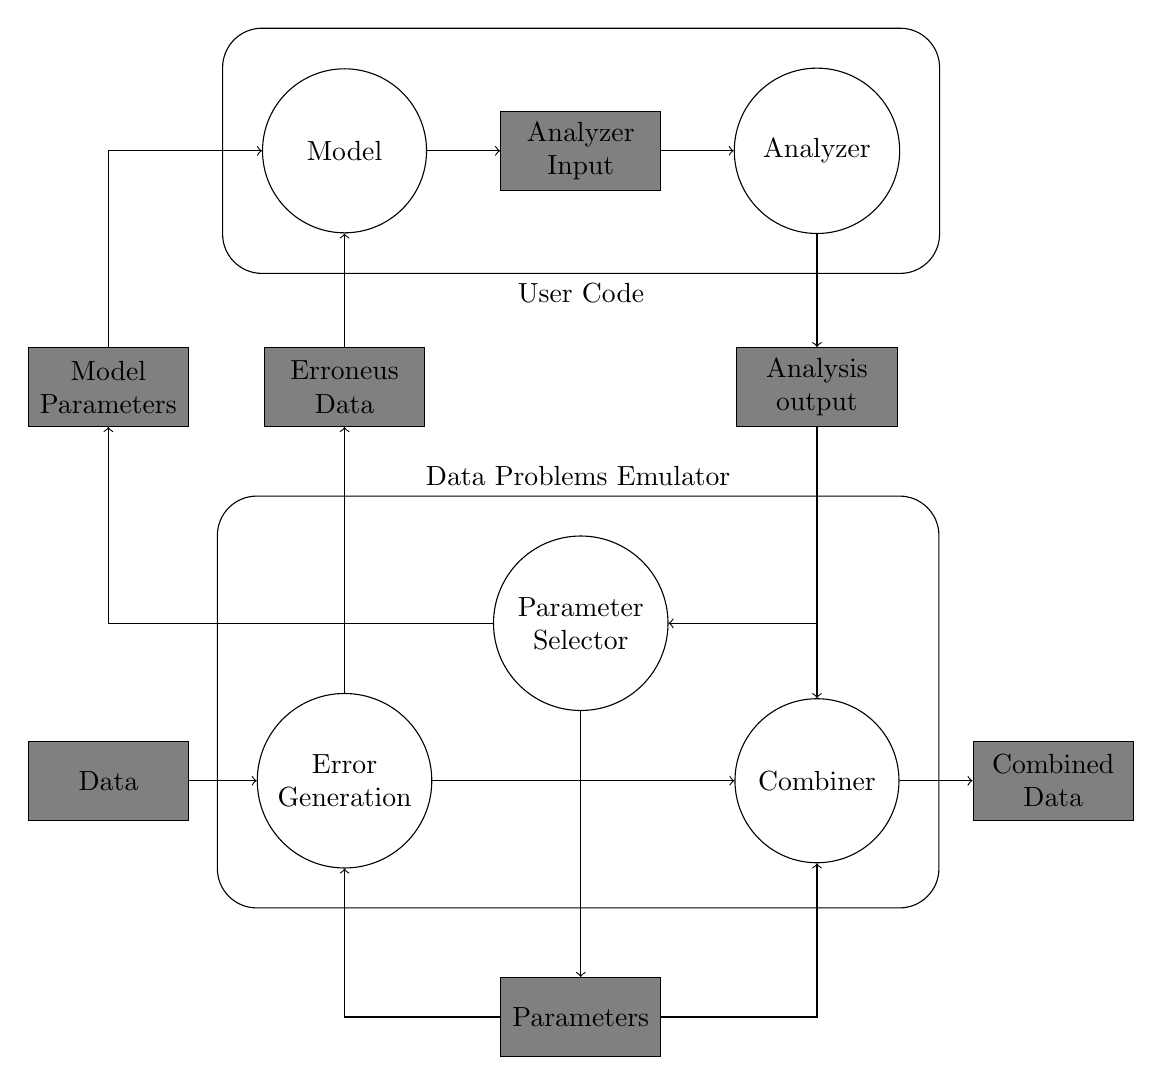
\begin{tikzpicture}[state/.style={circle, draw, align=center, minimum size=1cm, text width=1.8cm},file/.style={rectangle, fill=gray, draw, align=center, minimum size=1cm, text width=1.8cm}]
	% nodes
	\node[file] (data) {Data};%

	\node[state, right of=data, xshift=2cm] (error) {Error Generation};
	\node[file, above of=error, yshift=4cm] (errdat) {Erroneus Data}; %
	\node[file, left of=errdat, xshift=-2cm] (modpar) {Model Parameters}; %
	\node[state, above of=errdat, yshift=2cm] (model) {Model}; %
	\node[file, right of=model, xshift=2cm] (anain) {Analyzer Input}; %
	\node[state, right of=anain, xshift=2cm] (anlzr) {Analyzer}; %
	\node[file, below of=anlzr, yshift=-2cm] (anaout) {Analysis output}; %
	\node[state, below of=anain, yshift=-5cm] (parcho) {Parameter Selector}; %
	\node[state, below of=anaout, yshift=-4cm] (combiner) {Combiner}; %
	\node[file, right of=combiner, xshift=2cm] (res) {Combined Data}; %
	\node[file, below of=anain, yshift=-10cm] (param) {Parameters}; %

	% plate
	\node[label=above:Data Problems Emulator, draw, inner sep=.5cm, rounded corners=.5cm, fit=(error)(combiner)(parcho)] (dpemu) {}; %
	\node[label=below:User Code, draw, inner sep=.5cm, rounded corners=.5cm, fit=(model)(anain)(anlzr)] (user) {}; %

	% edges
	\draw [->] (data) -- (error);
	\draw [->] (error) -- (errdat);
	\draw [->] (error) -- (combiner);
	\draw [->] (errdat) -- (model);
	\draw [->] (modpar) |- (model);
	\draw [->] (model) -- (anain);
	\draw [->] (anain) -- (anlzr);
	\draw [->] (anlzr) -- (anaout);
	\draw [->] (anaout) -- (combiner);
	\draw [->] (combiner) -- (res);
	\draw [->] (param) -| (error);
	\draw [->] (param) -| (combiner);
	\draw [->] (anaout) |- (parcho);
	\draw [->] (parcho) -- (param);
	\draw [->] (parcho) -| (modpar);
\end{tikzpicture}
\end{document}
